\documentclass{beamer}
\mode<presentation>
\usepackage{amsmath}
\usepackage{amssymb}
%\usepackage{advdate}
\usepackage{adjustbox}
\usepackage{subcaption}
\usepackage{enumitem}
\usepackage{multicol}
\usepackage{mathtools}
\usepackage{listings}
\usepackage{minted}
% \usepackage{gvv}

\usepackage{tcolorbox}
\tcbuselibrary{minted,breakable,xparse,skins}



\definecolor{bg}{gray}{0.95}
\DeclareTCBListing{mintedbox}{O{}m!O{}}{%
  breakable=true,
  listing engine=minted,
  listing only,
  minted language=#2,
  minted style=default,
  minted options={%
    linenos,
    gobble=0,
    breaklines=true,
    breakafter=,,
    fontsize=\scriptsize,
    numbersep=8pt,
    #1},
  boxsep=0pt,
  left skip=0pt,
  right skip=0pt,
  left=25pt,
  right=0pt,
  top=3pt,
  bottom=3pt,
  arc=5pt,
  leftrule=0pt,
  rightrule=0pt,
  bottomrule=2pt,
  toprule=2pt,
  colback=bg,
  colframe=orange!70,
  enhanced,
  overlay={%
    \begin{tcbclipinterior}
    \fill[orange!20!white] (frame.south west) rectangle ([xshift=20pt]frame.north west);
    \end{tcbclipinterior}},
  #3,
}
\usepackage{url}
\def\UrlBreaks{\do\/\do-}
\usetheme{Boadilla}
\usecolortheme{lily}
\setbeamertemplate{footline}
{
  \leavevmode%
  \hbox{%
  \begin{beamercolorbox}[wd=\paperwidth,ht=2.25ex,dp=1ex,right]{author in head/foot}%
    \insertframenumber{} / \inserttotalframenumber\hspace*{2ex} 
  \end{beamercolorbox}}%
  \vskip0pt%
}
\setbeamertemplate{navigation symbols}{}

\providecommand{\nCr}[2]{\,^{#1}C_{#2}} % nCr
\providecommand{\nPr}[2]{\,^{#1}P_{#2}} % nPr
\providecommand{\mbf}{\mathbf}
\providecommand{\pr}[1]{\ensuremath{\Pr\left(#1\right)}}
\providecommand{\qfunc}[1]{\ensuremath{Q\left(#1\right)}}
\providecommand{\sbrak}[1]{\ensuremath{{}\left[#1\right]}}
\providecommand{\lsbrak}[1]{\ensuremath{{}\left[#1\right.}}
\providecommand{\rsbrak}[1]{\ensuremath{{}\left.#1\right]}}
\providecommand{\brak}[1]{\ensuremath{\left(#1\right)}}
\providecommand{\lbrak}[1]{\ensuremath{\left(#1\right.}}
\providecommand{\rbrak}[1]{\ensuremath{\left.#1\right)}}
\providecommand{\cbrak}[1]{\ensuremath{\left\{#1\right\}}}
\providecommand{\lcbrak}[1]{\ensuremath{\left\{#1\right.}}
\providecommand{\rcbrak}[1]{\ensuremath{\left.#1\right\}}}
\theoremstyle{remark}
\newtheorem{rem}{Remark}
\newcommand{\sgn}{\mathop{\mathrm{sgn}}}
\providecommand{\abs}[1]{\left\vert#1\right\vert}
\providecommand{\res}[1]{\Res\displaylimits_{#1}} 
\providecommand{\norm}[1]{\lVert#1\rVert}
\providecommand{\mtx}[1]{\mathbf{#1}}
\providecommand{\mean}[1]{E\left[ #1 \right]}
\providecommand{\fourier}{\overset{\mathcal{F}}{ \rightleftharpoons}}
%\providecommand{\hilbert}{\overset{\mathcal{H}}{ \rightleftharpoons}}
\providecommand{\system}{\overset{\mathcal{H}}{ \longleftrightarrow}}
	%\newcommand{\solution}[2]{\textbf{Solution:}{#1}}
%\newcommand{\solution}{\noindent \textbf{Solution: }}
\providecommand{\dec}[2]{\ensuremath{\overset{#1}{\underset{#2}{\gtrless}}}}
\newcommand{\myvec}[1]{\ensuremath{\begin{pmatrix}#1\end{pmatrix}}}
\let\vec\mathbf

\lstset{
%language=C,
frame=single, 
breaklines=true,
columns=fullflexible
}

\numberwithin{equation}{section}

\title{Presentation Template}
\author{B. Sai Likith Reddy \\ Dept. of Artificial Intelligence,\\IIT Hyderabad.}

\date{\today} 
\begin{document}

\begin{frame}
\titlepage
\end{frame}

\section*{Outline}
\begin{frame}
\tableofcontents
\end{frame}
\section{Problem}
\begin{frame}
\frametitle{Problem Statement}
%
 $\vec{P}\brak{5,-3}$ and $\vec{Q}\brak{3,y}$ are the points of trisection of the line segment joining $\vec{A}\brak{7,-2}$ and $\vec{B}\brak{1,-5}$. Theny equals

\end{frame}

%\subsection{Literature}
\section{Solution}
\subsection{section formula in matrix form}
\begin{frame}
\frametitle{Section formula}
If a point $\vec{R}$ divides the line segment joining the points $\vec{A}$ and $\vec{B}$ in the ratio $k:1$ then the point $\vec{R}$ can be found by using the section formula below
$$\vec{R}=\frac{\vec{A}+k\vec{B}}{1+k}$$
Now let $\vec{P}$ divides the Line segment in the ratio $1:k$ And then we will find $k$ if we know $k$ then we will know how $\vec{Q}$ divides the line segment and hence we can find the value of $y$
\end{frame}
\subsection{solving for k}
\begin{frame}
\frametitle{solving for k}
\begin{align}
\vec{P}&=\frac{k\vec{A}+\vec{B}}{k+1}\\
\myvec{5\\-3}&=\frac{k\myvec{7\\-2}+\myvec{1\\-5}}{1+k}
\end{align}
solving $x$ coordinate
\begin {align}
5\brak{1+k}&=7k+1
\end{align}
hence $k=2$
\end{frame}
\subsection{solving for $y$}
\begin{frame}
\frametitle{solving for $y$}
As the value of $k=2$\\
$\vec{Q}$ divides $\vec{AB}$ in the ratio $2:1$
\begin{align}
\myvec{3\\ y }&=\frac{\myvec{1\\-5}+\frac{1}{2}\myvec{7\\-2}}{1+\frac{1}{2}}
\end{align}
solving $y-$ coordinate
\begin{align}
\frac{3}{2}y&=-5-2\brak{\frac{1}{2}}
\end{align}
Therefore $y=-4$
\end{frame}
%\section{Plot}
\subsection{}
\begin{frame}[fragile]
\frametitle{Plot of the Points}
\begin{figure}[h!]


 \centering
    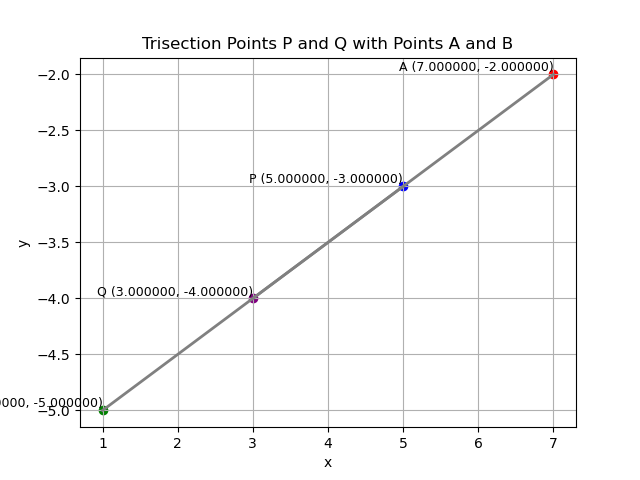
\includegraphics[width=0.7\textwidth]{figs/Figpresent.png}
\end{figure}
\end{frame}
\section{codes}
\subsection{C code to calculate points}
\begin{frame}[fragile,allowframebreaks]
\frametitle{generating points and the line}
\begin{mintedbox}{c}[break at=.8\textheight]
#include <stdio.h>
#include <stdlib.h>
#include <math.h>
#include "libs/matfun.h"
#include "libs/geofun.h"  // Include geofun.h for geometric operations

// Function to calculate trisection points P and Q
void calculate_trisection(double **A, double **B, double **Q, double **P) {
    // Trisection formulas
    Q[0][0] = (2 * B[0][0] + A[0][0]) / 3;  // P (1:2)
    Q[1][0] = (2 * B[1][0] + A[1][0]) / 3;

    P[0][0] = (B[0][0] + 2 * A[0][0]) / 3;  // Q (2:1)
    P[1][0] = (B[1][0] + 2 * A[1][0]) / 3;
}

// Function to generate points of trisection and write them to a file
void point_gen(double **A, double **B, const char *filename) {
    FILE *file = fopen(filename, "w");
    if (file == NULL) {
        printf("Error opening file.\n");
        return;
    }

    // Allocate memory for trisection points
    double **Q = createMat(2, 1);
    double **P = createMat(2, 1);

    // Calculate trisection points
    calculate_trisection(A, B, Q, P);

    // Write the points to the file
    fprintf(file, "Point A: (%lf, %lf)\n", A[0][0], A[1][0]);
    fprintf(file, "Point B: (%lf, %lf)\n", B[0][0], B[1][0]);
    fprintf(file, "Trisection Point P (1:2): (%lf, %lf)\n", P[0][0], P[1][0]);
    fprintf(file, "Trisection Point Q (2:1): (%lf, %lf)\n", Q[0][0], Q[1][0]);

    // Close the file
    fclose(file);

    // Free allocated memory
    freeMat(Q, 2);
    freeMat(P, 2);
}

int main() {
    // Initialize points A(7, -2) and B(1, -5)
    double **A = createMat(2, 1);
    double **B = createMat(2, 1);

    A[0][0] = 7;
    A[1][0] = -2;
    B[0][0] = 1;
    B[1][0] = -5;
    // Generate trisection points and save them to asgn2.dat
    point_gen(A, B, "asgn2.txt");
    // Free the allocated memory for A and B
    freeMat(A, 2);
    freeMat(B, 2);
    return 0;}
\end{mintedbox}
\end{frame}
\subsection{Plotting the figure using Python}
\begin{frame}[fragile,allowframebreaks]
\frametitle{Plotting the figure using Python}

\begin{mintedbox}{Python}[break at=.8\textheight]
import numpy as np
import matplotlib.pyplot as plt

# Load the points from the text file
points = []
with open("asgn2.txt", 'r') as file:
    for line in file:
        # Check if the line contains coordinates
        if '(' in line and ')' in line:
            # Isolate the part with the coordinates
            coords_part = line.split('(')[-1].split(')')[0].strip()  # Get part between '(' and ')'
            try:
                # Split the coordinates and convert them to floats
                x, y = map(float, coords_part.split(','))
                points.append((x, y))  # Append as a tuple
            except ValueError as e:
                print(f"Error converting coordinates in line: '{line.strip()}': {e}")

# Convert to numpy array for easier manipulation
points = np.array(points)

# Check if points were loaded correctly
if points.shape[0] < 4:
    raise ValueError("Data must contain at least four coordinates.")

# Extract the coordinates of points P, Q, B, and A
A = points[0]  # Trisection point Q
B = points[1]  # Trisection point P
P = points[2]  # Point B
Q = points[3]  # Point A


# Plot the points
plt.figure()

# Plot thick lines between points A and B, and P and Q
plt.plot([A[0], B[0]], [A[1], B[1]], color='gray', linewidth=2, label='Line AB')
plt.plot([P[0], Q[0]], [P[1], Q[1]], color='gray', linewidth=2, label='Line PQ')

# Plot the points A, B, P, and Q
plt.scatter(A[0], A[1], color='red', marker='o')  # Point A
plt.scatter(B[0], B[1], color='green', marker='o')  # Point B
plt.scatter(P[0], P[1], color='blue', marker='o')   # Point P
plt.scatter(Q[0], Q[1], color='purple', marker='o')  # Point Q

# Label the points with coordinates
plt.text(A[0], A[1], f"A ({A[0]:.6f}, {A[1]:.6f})", fontsize=9, verticalalignment='bottom', horizontalalignment='right')
plt.text(B[0], B[1], f"B ({B[0]:.6f}, {B[1]:.6f})", fontsize=9, verticalalignment='bottom', horizontalalignment='right')
plt.text(P[0], P[1], f"P ({P[0]:.6f}, {P[1]:.6f})", fontsize=9, verticalalignment='bottom', horizontalalignment='right')
plt.text(Q[0], Q[1], f"Q ({Q[0]:.6f}, {Q[1]:.6f})", fontsize=9, verticalalignment='bottom', horizontalalignment='right')

# Label the axes and add a title
plt.xlabel("x")
plt.ylabel("y")
plt.title("Trisection Points P and Q with Points A and B")
plt.grid(True)

# Save the resulting figure

plt.show()
	
	\end{mintedbox}
\end{frame}
\end{document}
